Effizienzsteigerung durch ICTs bedeutet, dass Werkzeuge bei Entscheidungen die den Ort, die Zeit und die Versorgung der Pflanzen betreffen Hilfe leisten. Dieses Kapitel beschäftigt sich mit drei Themen die mit der Unterstützung bei Entscheidungshilfen zu tun haben.

Es werden Arbeiten über Expertensysteme in der Landwirtschaft vorgestellt die aus den verfügbaren Daten und Zielen Empfehlungen zur Erreichung abgeben. Zusätzlich wird das Konzept des Life Cycle Assessment vorgestellt, welches durch ICTs effizient möglich wurde.

Durch die sich entwickelnde Technologisierung in Schwellenländern entwickeln sich dort neue Modelle wie Kleinbauern in der Entscheidungsfindung unterstützt werden können. Dazu werden Arbeiten vorgestellt die sich mit den verfügbaren Lösungen, deren Nutzen und den Entwicklungsmöglichkeiten beschäftigen vorgestellt.

\section{Automatisierte Entscheidungsfindung}

Die ganzheitliche Planung von Landwirtschaftsbetrieben ist ein komplexes Problem das makroskopische sowie mikroskopische Faktoren einbeziehen muss. Ein früher Ansatz um alle Umwelteinflüsse zu bewerten und die Ergebnisse in einer Optimierung der Prozesse einfließen zu lassen, ist das LCA (Life Cycle Assessment). Dabei werden alle Einflüsse in den Lebenszyklusphasen des Produkts bzw. Services identifiziert. Das Ergebnis dieses Identifikationsprozesses wird \textit{Inventory Table} genannt. Die identifizierten Bestände werden mittels \textit{Life Cycle Inventory Impact Assessment}, kurz LCIA oder LCI, auf Zahlen abgebildet die wiederspiegeln wie viel Einfluss die jeweiligen Faktoren haben. LCIA besteht aus vier Schritten:\cite{jour:Klopffer1997}

\begin{itemize}
	\item \textit{Klassifizierung}. Dazu werden die Eingabe- und Ausgabewerte die im \textit{Inventory Table} definiert zusammen gefasst.
	\item \textit{Charakterisierung}. Die im ersten Schritt zusammen gefassten Daten werden auf sg. \textit{impact categories}, zu Deutsch Einflusskategorien, abgebildet. Z.B. Sonnenstunden auf Maisertrag.
	\item \textit{Normalisierung}. Die in der Klassifizierung fest gestellten Einflusskategorien werden auf normalisierte Kategorien abgebildet. (Z.B. IPCC-Faktoren für Einflusskategorien der globalen Erwärmung.)
	\item \textit{Bewertung}. In diesem Schritt werden die klassifizierten Kategorien auf ihre Einflussmöglichkeit auf die Qualität des Produkts bzw. Services bewertet.
\end{itemize}

LCA ist in dem ISO-Standard 14044 enthalten.\cite{jour:Klopffer1997}

Eine andere Sicht auf die Datenquellen liefern Wang und Pang in \cite{jour:Wang2013}. Sie stellen ein System zur Evaluierung der nötigen Informationen, die für Entscheidungen der Landwirtschaft in Qiqihar nötig sind vor. Dabei liegt der Fokus auf Geschäftsanforderungen die den Rahmen vorgeben was mit den verfügbaren Mitteln erreicht werden. Dabei wird klar, dass die technischen Möglichkeiten, die vorhandene Nachfrage, die Umweltfaktoren sowie gesetzliche Vorlagen beachtet werden müssen.

\begin{figure}[h]
 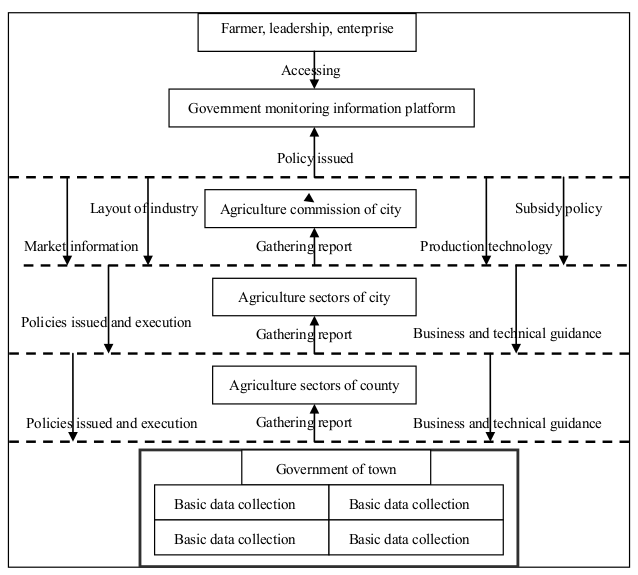
\includegraphics[scale=0.6,natwidth=\textwidth]{figures/designtools/businessrequirements.png}
 \centering
 \label{fig:fmishierarchy}
 \caption{Hierarchie von Datenquellen zu Entscheidungsträgern. \cite{jour:Wang2013}}.
\end{figure}

\subsection{Entwicklungen in der automatischen Auswertung}
Die Möglichkeit LCA in der Landwirtschaft einzusetzen wird in \cite{jour:Bellon-Maurel2014} beleuchtet. Zu Beginn des Papers gehen die Autoren auf Probleme herkömmlicher LCAs ein:
\begin{itemize}
	\item LCA als begleitende Maßnahme ist teuer da die Ermittlung der relevanten Daten aufwändig ist. Dementsprechend können nur große Betrieb LCA durchführen.
	\item Die herkömmlichen Messmöglichkeiten ermöglichen nur eine zeitverzögerte Reaktion die im Umfeld der Landwirtschaft zu Ausfällen führen können.
\end{itemize}

In ihrer Arbeit versuchen Bellon-Maurel, Short, Roux, Schulz und Peters den aktuellen Forschungsstand zusammen zu fassen und empfehlen den verstärkten Einsatz von ICTs um die LCI-Prozesse sie auf Kosten und Geschwindigkeit zu optimieren.\cite{jour:Bellon-Maurel2014}

Ein Faktor dessen Optimierungspotential durch Simulation erforscht wurde ist die maximale Lichteffizenz (\textit{maximum light efficency} $\varepsilon_{max}$. Wenquan, Yaozhang, Hao, Deyong und Haibo haben in \textit{Simulation of maximum light use efficiency for some typical vegetation types in China} gezeigt, dass der Fehlerintervall ihres Simulationsmodells klein genug ist um stabile und verlässliche Werte der Primärproduktion, kurz NPP, zu errechnen.  Damit kann bestimmt werden wo bestimmte Pflanzensorten angebaut werden können um den Ertrag zu maximieren. Die Basis für das Modell sind meterologische Daten, Vegetationskarten und vorhandene NPP-Daten.  \cite{jour:Zhu2006}

\begin{figure}[h]
 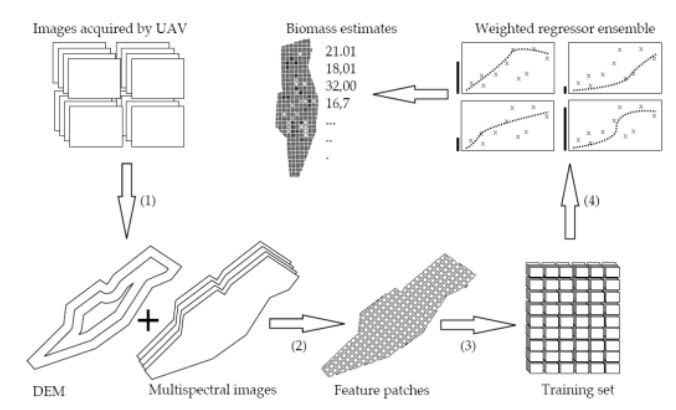
\includegraphics[scale=0.6,natwidth=\textwidth]{figures/designtools/uav_workflow.png}
 \centering
 \label{fig:uav_workflow}
 \caption{Hierarchie von Datenquellen zu Entscheidungsträgern. \cite{jour:Wang2013}}.
\end{figure}

Das in \cite{jour:Honkavaara2012} vorgestellte Drohnensystem basiert auf einem Algorithmus der vor Anwendung trainiert werden muss. Dieses Maschinenlernen erlaubt den Einsatz von im Vergleich zu Satellitenfotos kostengünstigen Material und eine rasche Auswertung der Daten. Der Prozess wird in Abbildung \ref{fig:uav_workflow} dargestellt.

\subsection{Entwicklungen in Schwellenländern}

In der dritten Welt zeichnet sich durch die Verbreitung von Smartphones einer durch das Mobilfunknetz gestützte Schwarmintelligenz ab. Damit wird die Menge der Kontakte eines Bauers zu einem Orakel, dass zu den Themen Wetter, Ertrag und Best-Practices befragt werden können.\cite{jour:Razaque2013} Die Bedeutung der Übertragung von Informationen für den Ertrag und damit der Effizienz wird in \cite{jour:State2013} untersucht. Das Ergebnis war, dass sowohl Internet wie Fernsehen und Radio zur Verfügung stehen. Interessant ist, dass in diesen Gebieten hauptsächlich Fernsehen- und Radioübertragung zur Verfügung stehen. Das Potential eine Schwarmintelligenz wie in \cite{jour:razaque2013} beschrieben aufzubauen ist vorhanden.

Die Entwicklung der Abdeckung des Mobilfunknetzes in Indien und die gestarteten Projekte zur Steigerung des Ertrags mittels Mobilfunkprojekten wird in \cite{article:Kokate2013} vorgestellt. Dabei werden Lösungen wie Krishi vorgestellt, welches es den Bauern ermöglichen soll per Telefonanruf Fragen bezüglich der Landwirtschaftsarbeit in normaler Sprache zu stellen. 

\section{Expertensysteme in der Planung}
Ein Expertensystem ist ein KI-Programm, dass zwei Rollen annehmen kann.
\begin{itemize}
	\item \textit{Decision Maker}, als Entscheidungsfinder ermittelt das Expertensystem die qualitativ beste Lösung für ein gegebenes Problem. Z.B. die Behandlung eines Patienten mit definierten Symptomen oder die optimale Bewässerung von Pflanzen.
	\item \textit{Oracle}, in diesem Fall dient das Expertensystem als Entscheidungshilfe in dem es gestellte Fragen beantwortet. 
\end{itemize}
Entscheidend für die Funktionalität des Expertensystems ist, dass ein Kausalmodell für die Problemdomäne gefunden wird, dieses zu einem quantitativen Entscheidungsmodell umgewandelt werden kann und daraus eine Entscheidung bzw. Antwort abgeleitet werden kann.\cite{book:Russell1995}

\begin{figure}[h]
 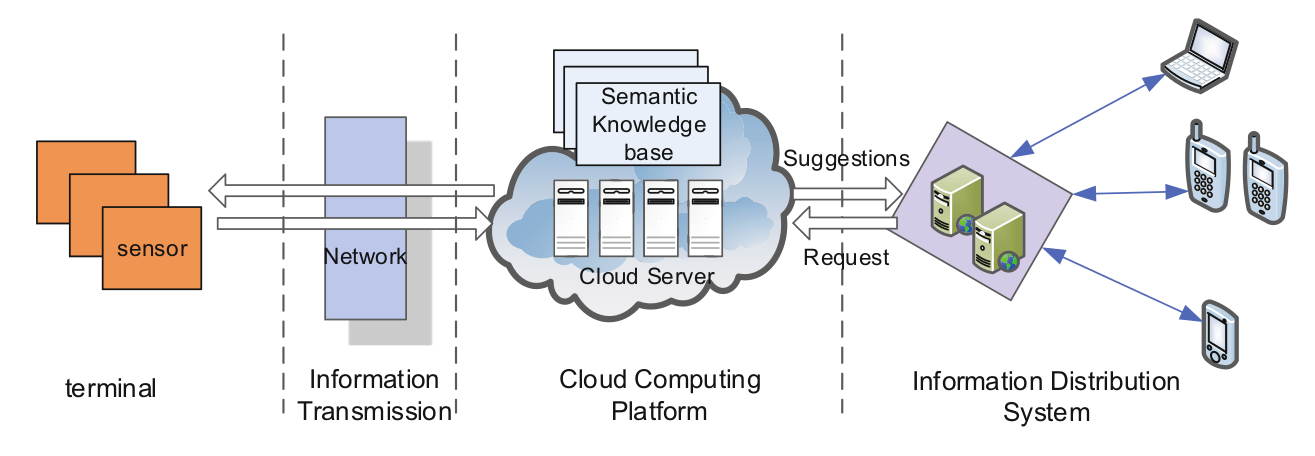
\includegraphics[scale=0.35,natwidth=\textwidth]{figures/designtools/cloud_iot_decisionmaker.png}
 \centering
 \label{fig:fmishierarchy}
 \caption{Architektur der Cloud-basierten Entscheidungshilfe.\cite{jour:Yuan2013}}.
\end{figure}

Lin, Nan, Li, Dongming, Bi und Chunguang stellen in \cite{jour:Lin2013} eine mögliche Architektur für ein System vor, dass bei der Planung und Pflege von Mais helfen soll. Dabei stellen sie folgende Best-Practices vor: 


\begin{itemize}
	\item Die Systemarchitektur und die Verwendung müssen als UML-Diagramme abgebildet werden. (Use-Case-Diagramme, Aktivitätsdiagramme, etc.)
	\item Die Datenbankstruktur muss als ER-Diagramm abgebildet werden.
	\item Die nötigen Objekte sollen mit der \textit{Object Definition Language}, kurz ODL, definiert werden.
	\item Die Verwendung der \textit{Framework Representation} um die Hierarchie und damit Kausalität von bestimmten Eigenschaften und Ereignissen abzubilden. (Z.B. ist ein Teil-Frame des Zustands von Gras dessen Halmzustand oder eine Erkrankung Teil des Disaster-Frames.)
\end{itemize}

Das in \cite{jour:Romeo2013} vorgestellte Expertensystem dient dazu, die grüne Färbung der Blätter zu bestimmen. Dies kann z.B. dazu genutzt werden um die Wasserversorgung bedarfsorientiert zu gewährleisten.

Um die Entscheidungsfindung besser in puncto Effizienz und Geschwindigkeit zu machen wird in \cite{jour:Yuan2013} ein Cloud basiertes System vorgestellt. 

Yuan, Zeng und Zhang stellen in ihrer Arbeit ein Expertensystem auf Basis eines Wissensbasierten System vor. Dabei werden Daten aus einem Sensornetzwerk als Ontologien abgebildet. Diese werden in der Cloud gespeichert. In der Cloud sitzt das Expertensystem, dass in der Lage ist Entscheidung zu treffen. Die Gesamtheit dieses Systems wird \textit{Semantic Technology} genannt.\cite{jour:Yuan2013}

Semantic Technology, kurz ST, bezeichnet die Technologie die vorhandene Daten als  Ontologien aufbereiten um automatisiert Entscheidung ableiten zu können. Die in \cite{jour:Liu2012} vorgestellte Architektur ST die ein Expertensystem und ein Sensornetzwerk verknüpft wird von Yuan, Zeng und Zhang wiederverwendet.

\section{Planungswerkzeuge}

Dieses Unterkapitel beschäftigt sich mit Systemen die bei der strategischen Planung und der kurzfristigen Entscheidungsfindung Unterstützung anbieten. Dazu werden exemplarisch Arbeiten vorgestellt für mittellose Kleinbetriebe und große industrielle Betriebe.

\subsection{DSS in der Landwirtschaft}
DSS (Decision Support Systems) ist der Oberbegriff für Planungswerkzeuge die dazu dienen halbautomatisch Abläufe und Pläne zu optimieren. In \cite{jour:Liu2013} wird ein DSS vorgestellt, das mehrere Analysemodelle integriert und in dem Gebiet Xuchang evaluiert wurde.

\begin{figure}[h]
 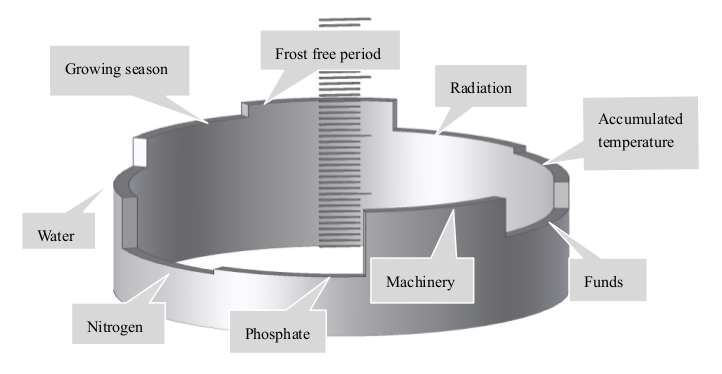
\includegraphics[scale=0.5,natwidth=\textwidth]{figures/designtools/dss_research.png}
 \centering
 \label{fig:dss_datasource}
 \caption{Die verschiedenen Eingabewerte die im RADDSS berücksichtigt wurden.}
\end{figure}

Das RADSS (Regional Agriculture Decision Support System) nimmt finanzielle Rahmenbedingungen sowie die vorhandenen Wetterbedingungen, siehe Abbildung \ref{fig:dss_datasource}, zur Berechnung von Vorhersagen. Lt. Liu konnten damit Kosten verringert und der Ertrag gesteigert werden. Die Evaluierung der Ergebnisse wird dazu jährlich durchgeführt.

In \cite{jour:Wenkel2011} wird LandCaRe-DSS vorgestellt, ein DSS zur Optimierung von von Betrieben um auf Veränderungen des Wetters durch den Klimawandel zu reagieren. In dieser Arbeit zeigt Wenkel, dass an DSS geforscht wird die komplexe globale Verhältnisse in die Ergebnisfindung mit einbeziehen können und dass es notwendig ist, bessere Modelle für Umwelteinflüsse zu finden.

Dutta stellt in \cite{jour:Dutta2014} ein DSS vor das auf einem Framework basiert dessen Lernalgorithmus mit verschiedenen Datenquellen arbeiten kann. Das Framework heißt i-EKbase (Intelligent Environmental Knowledgebase).

\subsection{Effizienz im Flottenmanagement}
In großen Landwirtschaftsbetrieben spielt das effiziente Flotten-Management eine bedeutende Rolle. In \cite{jour:Sorensen2010} wird eine ganzheitliche Lösung experimentell geprüft die zeigen soll welche Verbesserungen von einem System zu erwarten sind das sowohl die Auslastung der einzelnen Geräte, Wege für die Maschinen und die operationale Effizienz optimieren soll.

\begin{figure}[h]
 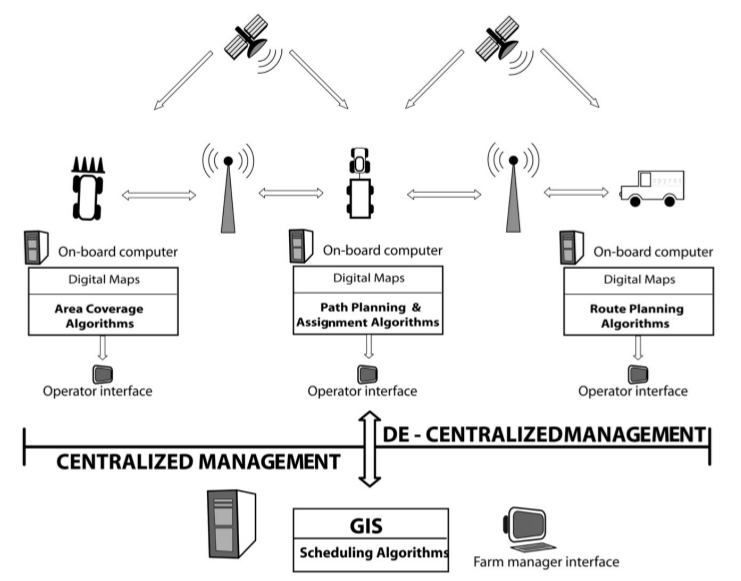
\includegraphics[scale=0.5,natwidth=\textwidth]{figures/designtools/centralized_vs_decentralized.png}
 \centering
 \label{fig:centralized_vs_decentralized}
 \caption{Vergleich zwischen zentralem und dezentralem Planungsansatz im Flotten-Management.}
\end{figure}

Abbildung \ref{fig:centralized_vs_decentralized} zeigt den Unterschied zwischen einem zentralen und einem dezentralen Ansatz. Während im zentralen Ansatz die Planung in einem leistungsstarkem System geschieht, wird im dezentralen Einsatz die Planung auf alle Akteure verteilt. Der Vorteil des verteilten Systems ist, dass Sensoren auf den Akteuren zeitnah Informationen in die Planung einfließen lassen können, der Nachteil ist, dass die Akteure untereinander kommunizieren müssen um eine Entscheidung zu finden. S\o rensen sieht keine Alternative zu der Verwendung der Sensoren auf den Maschinen und empfiehlt im Bereich Balancierung zwischen Kommunikationsaufwand und Verwertung vorhandener Informationen (z.B. aus GIS-Systemen) weiter zu forschen.

\subsection{Planungswerkzeuge für Freiluftunternehmen}
Im Gegensatz zu Glashäusern sind Felder der Umwelt schutzlos ausgeliefert. Das bedeutet, dass sich die Umweltfaktoren schnell ändern können und nicht alle Faktoren ausgeglichen werden können. (z.B. können Pflanzen nicht gegen Hagel geschützt werden.)

Den Einsatz von Ingenieurswerkzeugen um einen bestimmten Ertrag (z.B. Ernte, Kohle, etc.) zu produzieren werden \textit{Open Air Engineering}-Prozesse genannt. Diese Arbeiten zeichnen sich dadurch aus, dass im Betrieb eine Menge von verschiedenen Fahrzeugen und Arbeitern zusammen wirken müssen. (z.B. Mähdrescher, Traktoren um Pflügen, Traktoren um Wasserpumpen zu betreiben, etc.)

In \cite{conf:Valckenaers2011} stellen Valckenaers und Belle auf ein Planungskonzept für Open Air Engineering Prozesse vor. Die Basis ist eine Umsetzung der PROSA-Architektur um die im Prozess beteiligten Akteure als Agenten zu modellieren. Diese Agenten können in einer Simulation getestet werden um Probleme in der Ausführung erkennen zu können.

Für kleine Betriebe wird in \cite{conf:Lantzos2013} eine Android-Anwendung vorgestellt die kostengünstig und ohne Materialeinsatz Planungsaufgaben erledigen soll. Die Anwendung dient sowohl zur Kostenrechnung für Material und Personal wie auch Vermessung der Anbaufläche.